\chapter{Experimental}
\label{experimental}

In this chapter the setup and qualification process of the the optical and mechanical system is explained.  







\section{The Artificial Eye}
The test setup, which will be described in the following section, was the first physical assembly of the Artificial Eye. It was built after the design, which Chanal described in his report and was the base for the development process described in this chapter. This initial test setup is the first of three development steps described in this thesis. It is marked as orange-bordered in figure \ref{ChainTestSetup}.

\begin{figure}[h]
\begin{center}
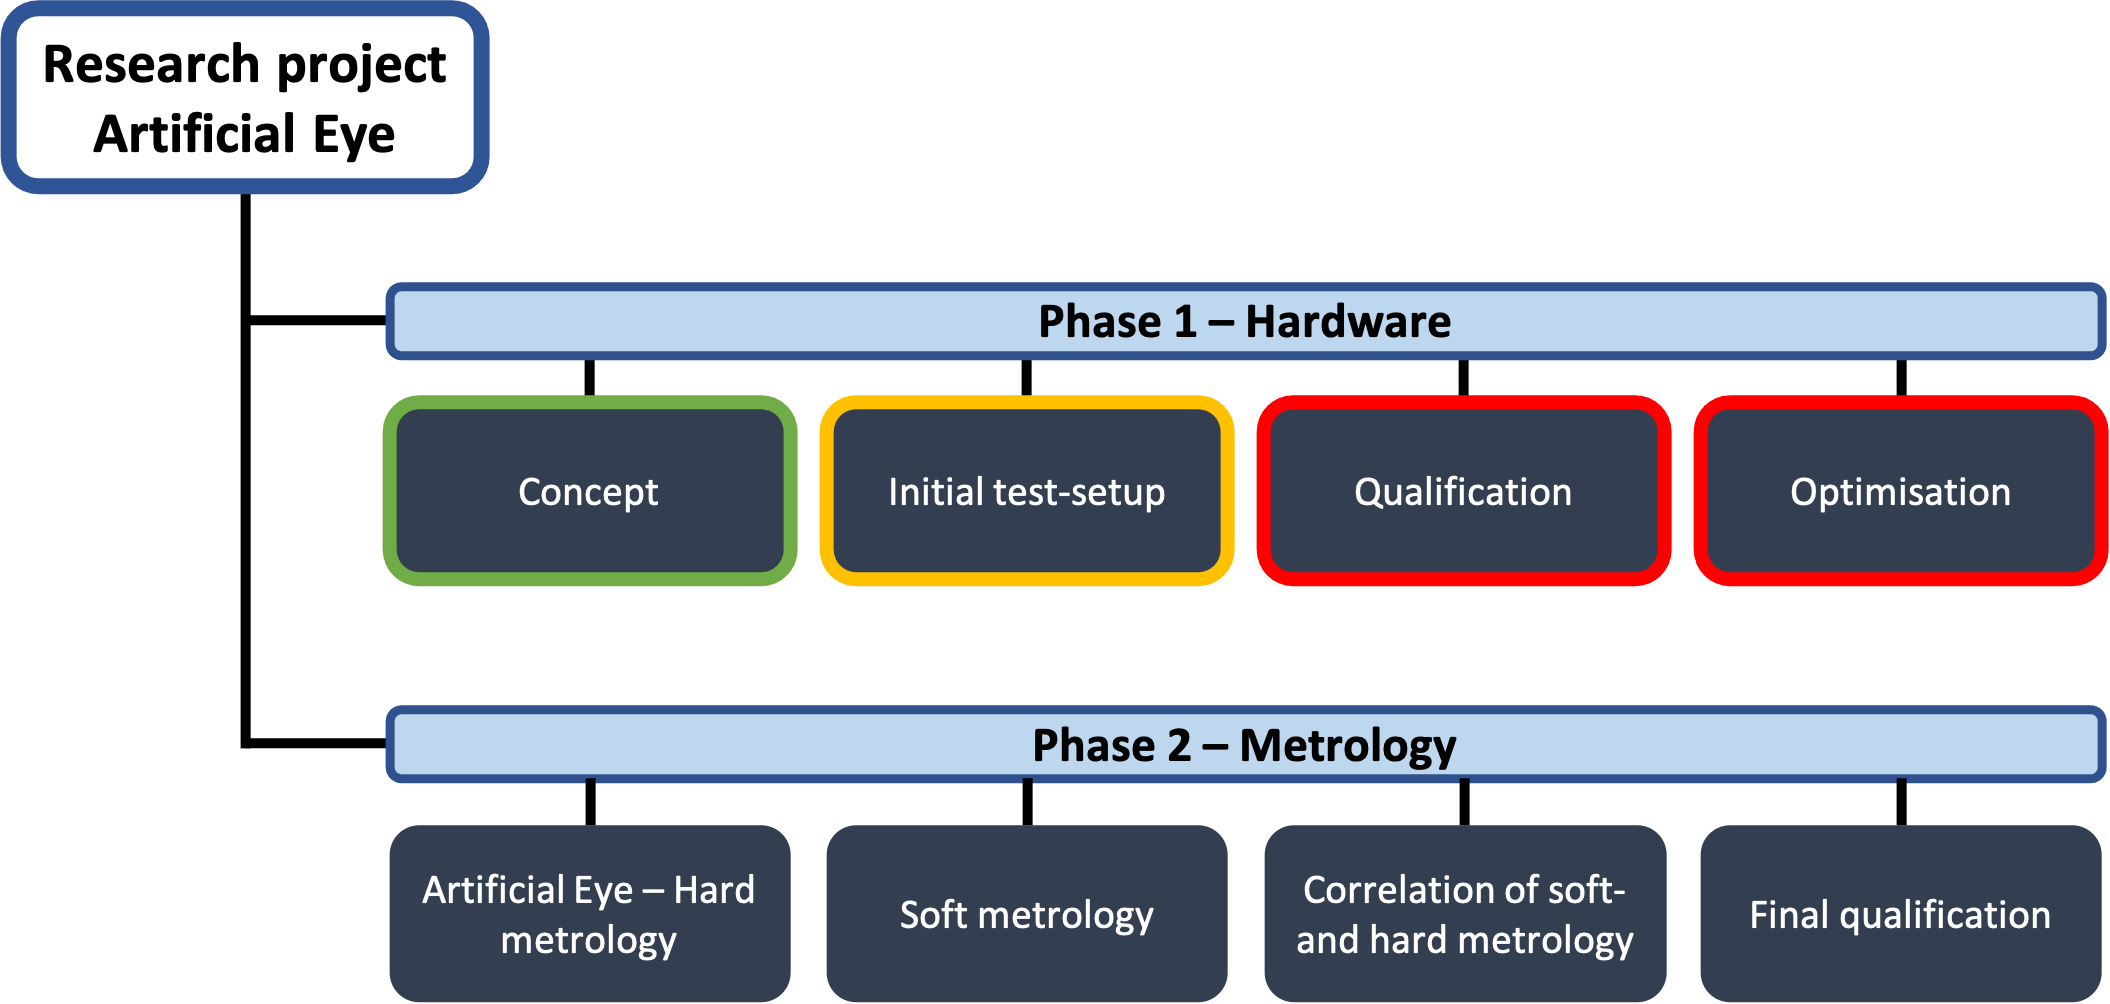
\includegraphics[width=12cm]{Pictures/ChainTestSetup}
\caption[Overview over the development process - Initial test setup]{Overview over the development process - Initial test setup: Green - Completed, Orange - In work, Red - Open}
\label{ChainTestSetup}
\end{center}
\end{figure}


\subsection{Optical system}
The optical system of the Artificial Eye is mostly built to represent the setup of the human eye. Similar to the human eye, the light enters the Artificial Eye through a lens, which focuses the image of the sample on to the light sensors. This lens is a machine vision lens produced by Tamron (see Appendix \ref{AppLoC}) and has a fixed focal length of 75mm and an entry pupil size of 25.5mm. As the human eye, the Artificial Eye has different sensors for colour and light intensity. In the Artificial Eye, these sensors are represented by a system of four digital CMOS cameras with a resolution of 2448 by 2048 pixels and a global shutter. The selected cameras are from the the 5 mega pixel Phoenix series from the manufacturer "Lucid Cameras" (see Appendix \ref{AppLoC}). All four cameras are similar in their sensor and electronics, but differ in the filter pattern which is applied to the physical pixels. On one of the four cameras a standard Bayer-pattern is applied to create a coloured image in software. The three other cameras also have a pattern of filters applied to their physical pixels. But instead of a colour filter this pattern selects different polarisation states of the incoming light. The filter pattern is shown in figure \ref{PHX050S} and filters the incoming light for linear polarisation with the orientation of 90°, 45°, 135° and 0°. In addition to the camera system, the incoming light is also picked up by a Czerny-Turner spectrometer from the company Thorlabs (see Appendix \ref{AppLoC}) to be used as a reference for the camera system.\\
As shown in the digram on the left side of figure \ref{AE_Setup}, the light has to pass through a quarter wave-plate after the lens. The wave-plate will turn right hand polarised light into a 45° linear polarised light and left hand circular polarised light into 135° linear polarised light. Linear polarised light with an orientation of 0° or 90° relative to the fast axis of the wave-plate will not be affected. Next, the light beam is passed through a system of non polarising beamsplitters with a transmission rate of 50/50. The beamsplitter equally distribute the light to the three polarised cameras and to the non-polarising camera as well as the spectrometer. The information of the polarisation of the light can later be used to calculate the surface roughness as well as the material thickness of transparent materials. It is important to note, that similar to an interferometer, a whole section of the sample can be measured at once. This saves time on the one hand, but on the other hand lowers the probability to miss important features of the surface.

\begin{figure}
\begin{center}
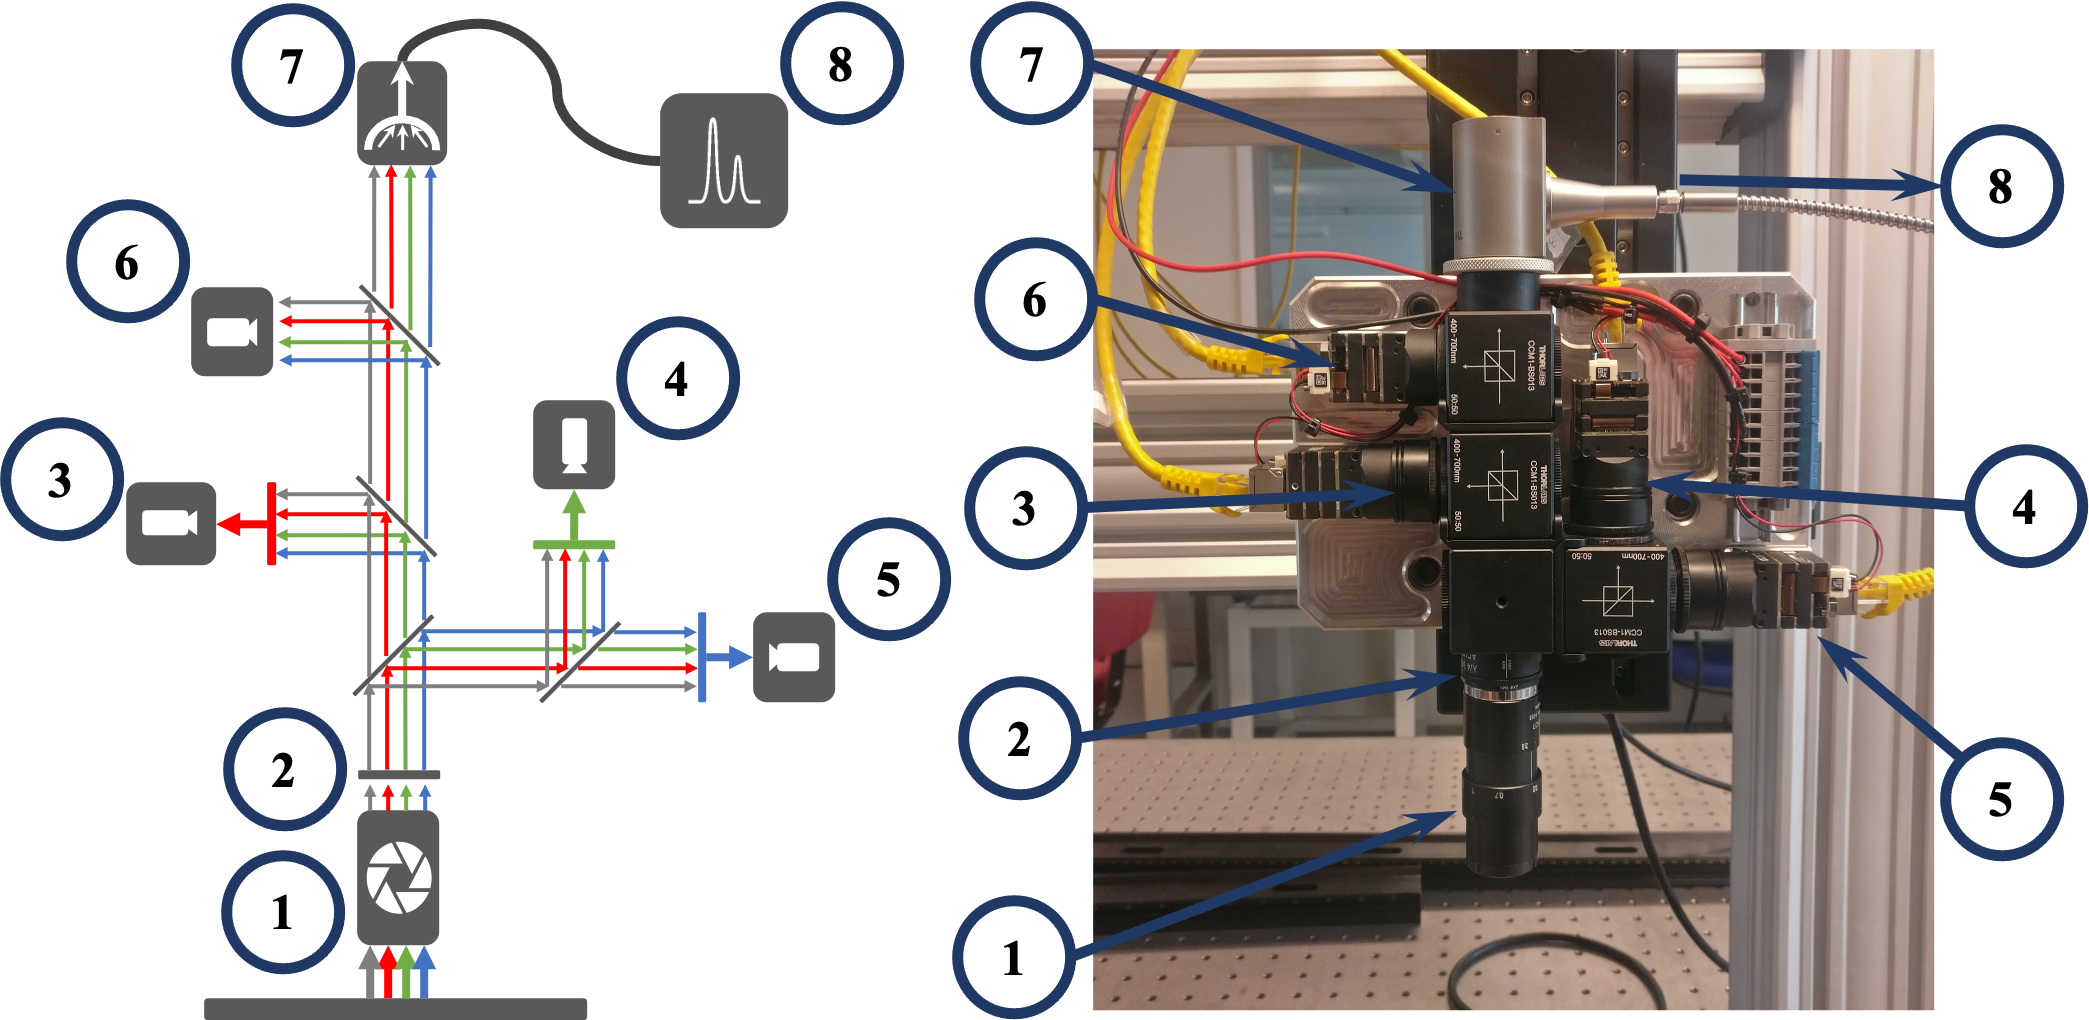
\includegraphics[width=12cm]{Pictures/AE_Setup}
\caption[Schema of the Artificial Eye]{Schema of the Artificial Eye: 1 - Machine vision lens, 2 - Quarter wave plate, 3 - Red filtered camera, 4 - Green filtered camera, 5 - Blue filtered camera, 6 - RGB camera, 7 - Fibre coupler, 8 - Spectrometer}
\label{AE_Setup}
\end{center}
\end{figure}

\begin{figure}
\begin{center}
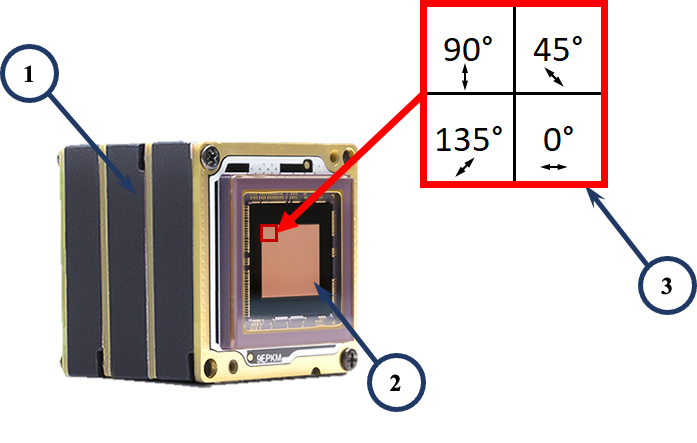
\includegraphics[width=12cm]{Pictures/LucidPHX505s}
\caption[Picture of the Lucid PHX050S Polarised Camera]{Picture of the Lucid PHX050S Polarised Camera\cite{Labs}: 1 - PHX050S Camera, 2 - CMOS Sensor, 3 - Detail of the polarisation pixel pattern}
\label{PHX050S}
\end{center}
\end{figure}

In order to represent the cones of the human eye, which are responsible for the colour vision in the human eye and only see a very small portion of the electromagnetic spectrum, the light is filtered similarly before being picked up by the polarised cameras. This is done with bandpass filters with a Bandwidth (FWHM) off 10 nm, with a CWL of 420 nm for the blue, 530 nm for the green and 620 nm for the red spectrum. This part of the Artificial Eye is responsible for colour-metric measurements, similar to a spectrophotometer. 


\subsection{Mechanical system}
The mechanical system built for the Artificial Eye consists of three linear travel stages arranged as a 3-axis cartesian motion system. The three axes are arranged in a way that the measurement setup is only moving in one axis, in Z. This has the advantage, that the heavy camera system only needs to move when it is necessary to adjust the focus. The sample will then be placed on the two remaining axes which are arranged as "X-Y table". Both, X-Y table and Z axis are mounted as shown in figure \ref{MotionSystem} on top of an optical table (to read more about optical tables see Appendix \ref{AppendixAdditionalTopics}).\\
It was necessary to calibrate the motion system to ensure that the X and Y axis are mounted in 90° angle to each other. Further, the Z axis with the measurement setup needed to be mounted perpendicular to the X-Y Table. This calibration was done with the help of the camera system of the Artificial Eye.\\
First the Z axis was calibrated. This was done by focusing the camera system on a specific point on the optical table. As a next step the camera system was moved towards the optical table and the focus of the lens was adjusted until the camera image was sharp again. As soon as the Z axis was perpendicular to the surface of the optical table, the point of interest remained in the center of the Field of View (FOV) during movements in Z.\\
For X and Y, the system was focused onto one edge of the X-Y table. One of the axes was then moved by 20 mm. After the movement, the position of the edge was compared to its initial position. If the table only moved along the axis of intended movement, the rotation of the moved axis (relative to the rest of the system) could be declared as good. Was the edge slightly wandering off into one direction perpendicular to the direction of movement, the moved axis was slightly rotated around the Z axis and needed to be corrected. This process was repeated multiple times for both, X and Y axis in order to complete the calibration.

\begin{figure}
\begin{center}
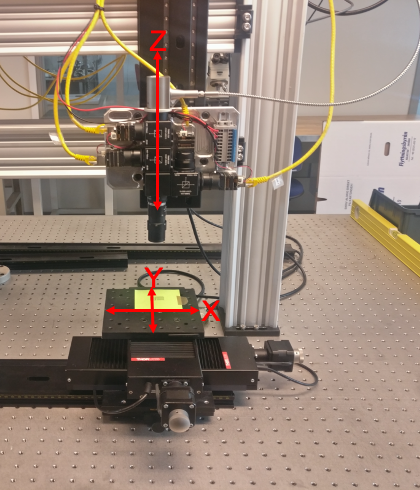
\includegraphics[width=12cm]{Pictures/MotionSystem}
\caption[Picture of the motion system of the Artificial Eye]{Picture of the motion system of the Artificial Eye}
\label{MotionSystem}
\end{center}
\end{figure}


\subsection{Electrical system}
In order to operate the Artificial Eye and acquire data from the camera system and the spectrometer a power and data connection needed to be provided to the setup. To avoid timing problems with the camera system and run the cameras at a cooler temperature, the decision was made to not to use the POE (Power over Ethernet) capability of the cameras. The camera system was powered with an external 24V Power Supply.\\ 
Figure \ref{ElectricalSetup} shows the overview of the electronic circuit:

\begin{enumerate}
	\item \textbf{Schuko plug type F:} The Schuko plug is connected to an 230 VAC power outlet to power the circuit.
	\item \textbf{Phoenix Contact Mini PS 100:}The power supply converts 230 VAC to 24 VDC. It has a maximum power output of 48 W. It can operate in a temperature range from -25 °C to 60 °C.\cite{RSComponents}
	\item \textbf{Cat. 5E Ethernet cable:} The Cat. 5E transfers the data from the camera system and the USB Hub to the Ethernet switch. Both ends have a male RJ45 connector.
	\item \textbf{Camera System:} The camera system can be powered with both, power over Ethernet (POE) or 12 VDC to 24 VDC external power. To avoid interferences in the Ethernet cable when using POE the camera system was powered with an external source of 24 VDC. As data connection a 100 MBps (Million Bits per second) ethernet connection was used.
	\item \textbf{Thorlabs CCS 100/M Spectrometer:} The CCS100/M is the metric version of Thorlabs compact CCD spectrometer series. It uses a rugged Czerny-Turner spectrometer design with no moving parts. The wavelength range of the spectrometer is 350 nm to 700 nm with a spectral accuracy $<$0.5 nm at 435 nm. The spectrometer was connected to the USB Hub with a USB-A to Mini USB-B Cable. The input light was coupled into a optical fibre with a reflective coupler.\cite{ThorlabsCCS}
	\item \textbf{Thorlabs reflective coupler:} The RC12FC-P01 is a reflective collimator and coupler by the company Thorlabs. It can be used for a wavelength range from 450 nm to 2 $\mu$m and has a input/output opening of 12 mm.\cite{ThorlabsCoupler}
	\item \textbf{DIGI 14 Port USB Hub:} The 14 port USB Hub manufactured by the company DIGI (see Appendix \ref{AppLoC}) offers 14 USB2.0 or 3.1 ports for extension over Ethernet. It can be mounted in a standard 19" server rack. 
	\item \textbf{MikroTik 24 Port Ethernet Switch:} The MikroTik (see Appendix \ref{AppLoC}) 24 Port Ethernet switch is the central point of the Ethernet network. It connects all devices to the host computer and manages their communication.
\end{enumerate}

\begin{figure}
\begin{center}
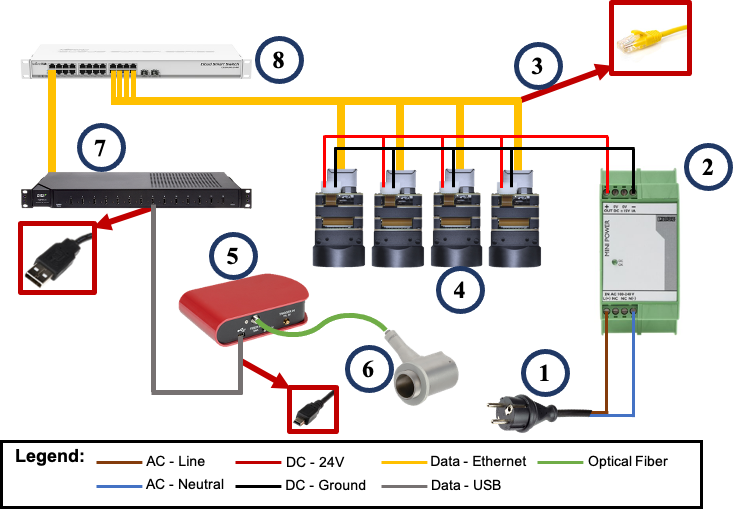
\includegraphics[width=12cm]{Pictures/Electrical Setup}
\caption[Electronic Circuit of the Artificial Eye:]{Electronic Circuit of the Artificial Eye: 1 - Schuko plug type F\cite{MuellerPlastik}, 2 - Phoenix Contact Mini PS 100\cite{RSComponents}, 3 - Cat5e Ethernet Cable\cite{ComputerCableStore}, 4 - Camera system\cite{Labs}, 5 - Thorlabs CCS 100/M Spectrometer\cite{ThorlabsCCS}, 6 - Thorlabs reflective coupler\cite{ThorlabsCoupler}, 7 -  DIGI 14 Port USB Hub\cite{DIGI}, 8 - MikroTik 24 Port Ethernet Switch\cite{MikroTik}}
\label{ElectricalSetup}
\end{center}
\end{figure}

\subsection{Software}
The acquisition, processing and evaluation of the data collected by the camera system and the spectrometer was done with a program created in LabVIEW (see Appendix \ref{appendixSoureCode}). This could be compared to the function of the human brain, which also acquires, processes and evaluates the pictures collected by the eyes. In order to have a clearly structured, maintainable as well as expandable software, the program was split into multiple subprograms. The so called "Sub-VI's" all have their own specific task such as configuring the camera system, processing the images or saving the resulting data.\\

\begin{figure}
\begin{center}
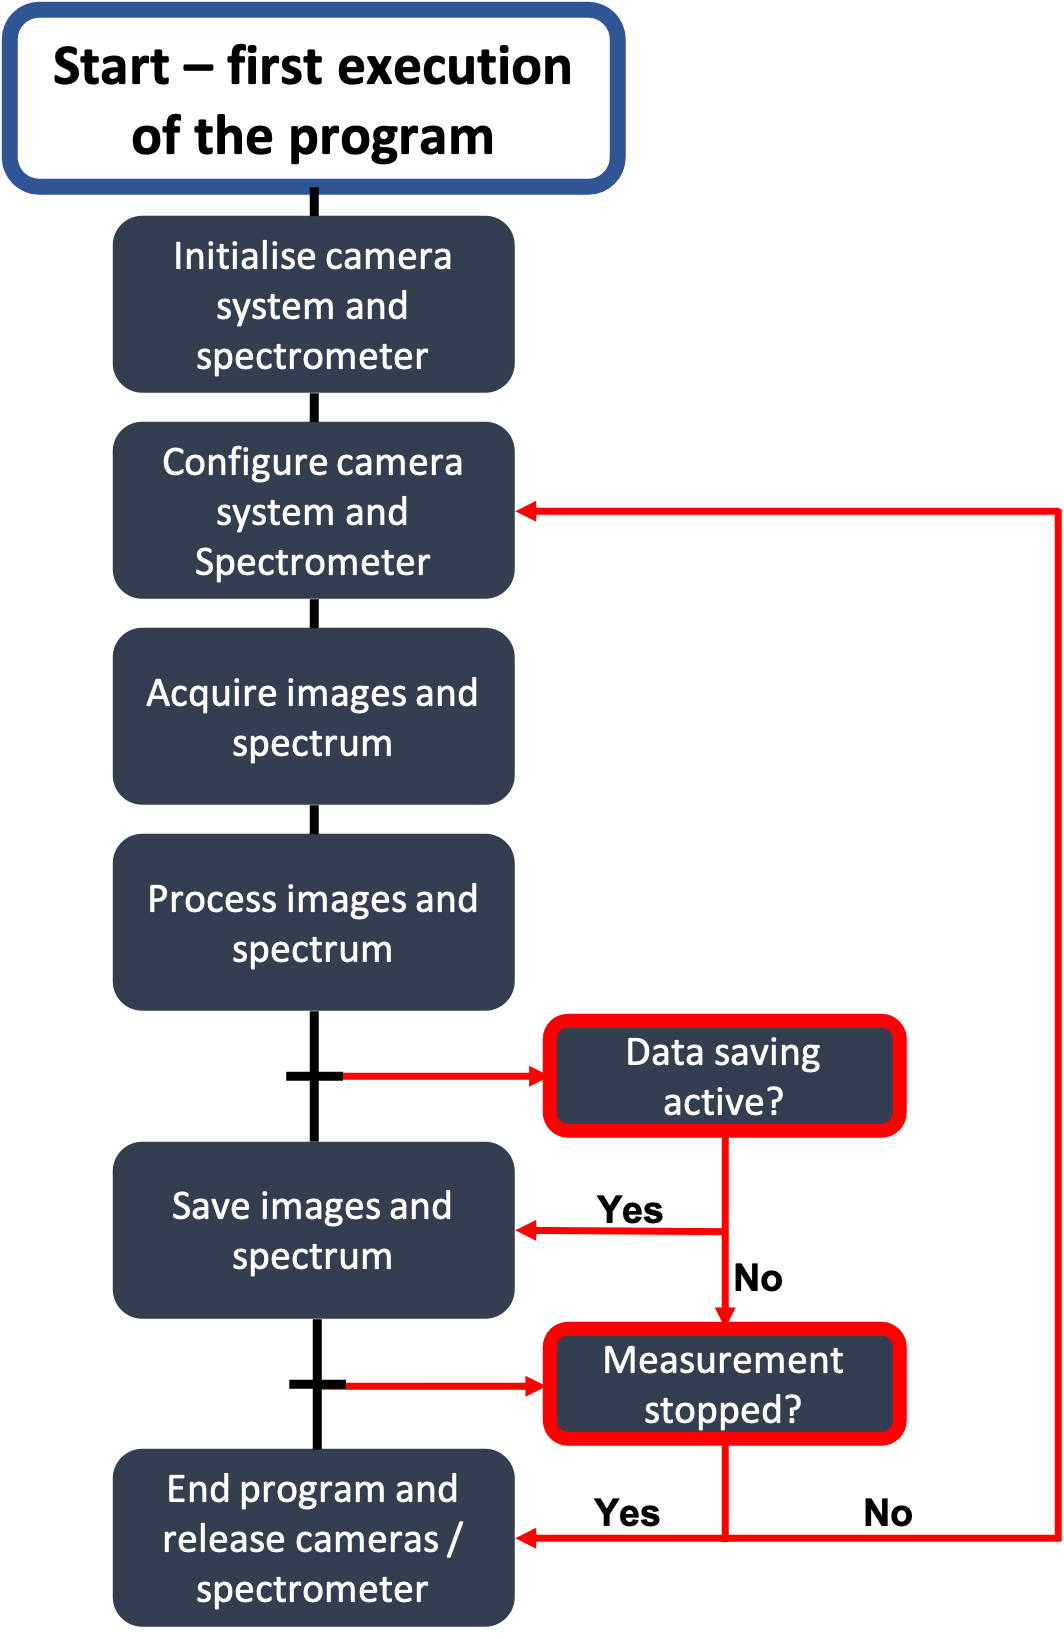
\includegraphics[width=12cm]{Pictures/MainVI}
\caption[Flowchart of the LabVIEW program]{Flowchart of the Labview program}
\label{MainVI}
\end{center}
\end{figure}

A flowchart of the Program is shown in figure \ref{MainVI}:

\begin{enumerate}

	\item \textbf{CamInit.vi and SpecInit.vi:} The subprograms "CamInit" and "SpecInit.vi" are responsible to initialise the connection to the camera system and the spectrometer. They house all functions needed to establish the serial connection via Ethernet to the five devices. These functions are only executed once, at the start of the program.
	\item \textbf{CamConf.vi:} This subprograms configure the acquisition parameters for the camera system. It is responsible to send the acquisition parameters such as exposure time, analogue gain, field of view to the devices. To be able to adjust these parameter while the program is running, this subprogram has to be executed every acquisition cycle.
	\item \textbf{CamAcqu.vi and SpecAcqu.vi:} The acquisition of the images happens in the subprograms "CamAcqu.vi" and "SpecAcqu.vi". In order to lower the traffic on the Ethernet connection, the acquisition of the data is handled separately for each of the cameras and the spectrometer. This means that the data acquisition of camera 1 has to be finished before camera 2 is allowed to send data. 
	\item \textbf{Processing.vi:} "Processing.vi" is the core function of the the Artificial Eye software. It takes the raw images as inputs and outputs the processed images. This subprogram corrects mirrored and flipped images caused by the beamsplitters and mounting of the cameras.
	\item \textbf{ImSave.vi:} As last step the acquired images as well as the spectrum are saved to the hard drive of the computer. This is done to be able to evaluate the data in post processing with programs like MATLAB. The images are saved as complete 2048x2048 16 bit unsigned integer binary file. Further, each of the images is split and saved as a smaller partial image with a resolution of 1024x1024. These images only contain one polarisation or in case of the RGB camera one of the four intensities produced by the bayer pattern. This is done by splitting the image into four before saving. The spectrometer data will be saved as a .csv (coma-separated values) file. In order to not fill up the hard drive with useless data, saving can be activated or deactivated. When active the LabVIEW function will create a new folder, marked with date and time, for each new acquisition cycle. Data saving is turned off by default.
	\item \textbf{Main.vi:} The program "Main.vi" is responsible to control all subprograms. This program will be used by the operator. It will run the device configuration, data acquisition, data processing and saving in an infinite loop, until interrupted by the operator.
	\item \textbf{Visualisation:} The front panel of the program Main.vi represents the GUI which will be used by the operator of the system. It will show a live view of the camera and spectrometer data and enables the operator to interact with the system. It offers the controls to change the gain and exposure time for each camera and set the integration time of the spectrometer. Further it enables the user to start and stop the program as well as to enable and disable the saving feature. The latest version of the Main.vi front panel is shown in figure \ref{Frontpanel}.
\end{enumerate}

\begin{figure}
\begin{center}
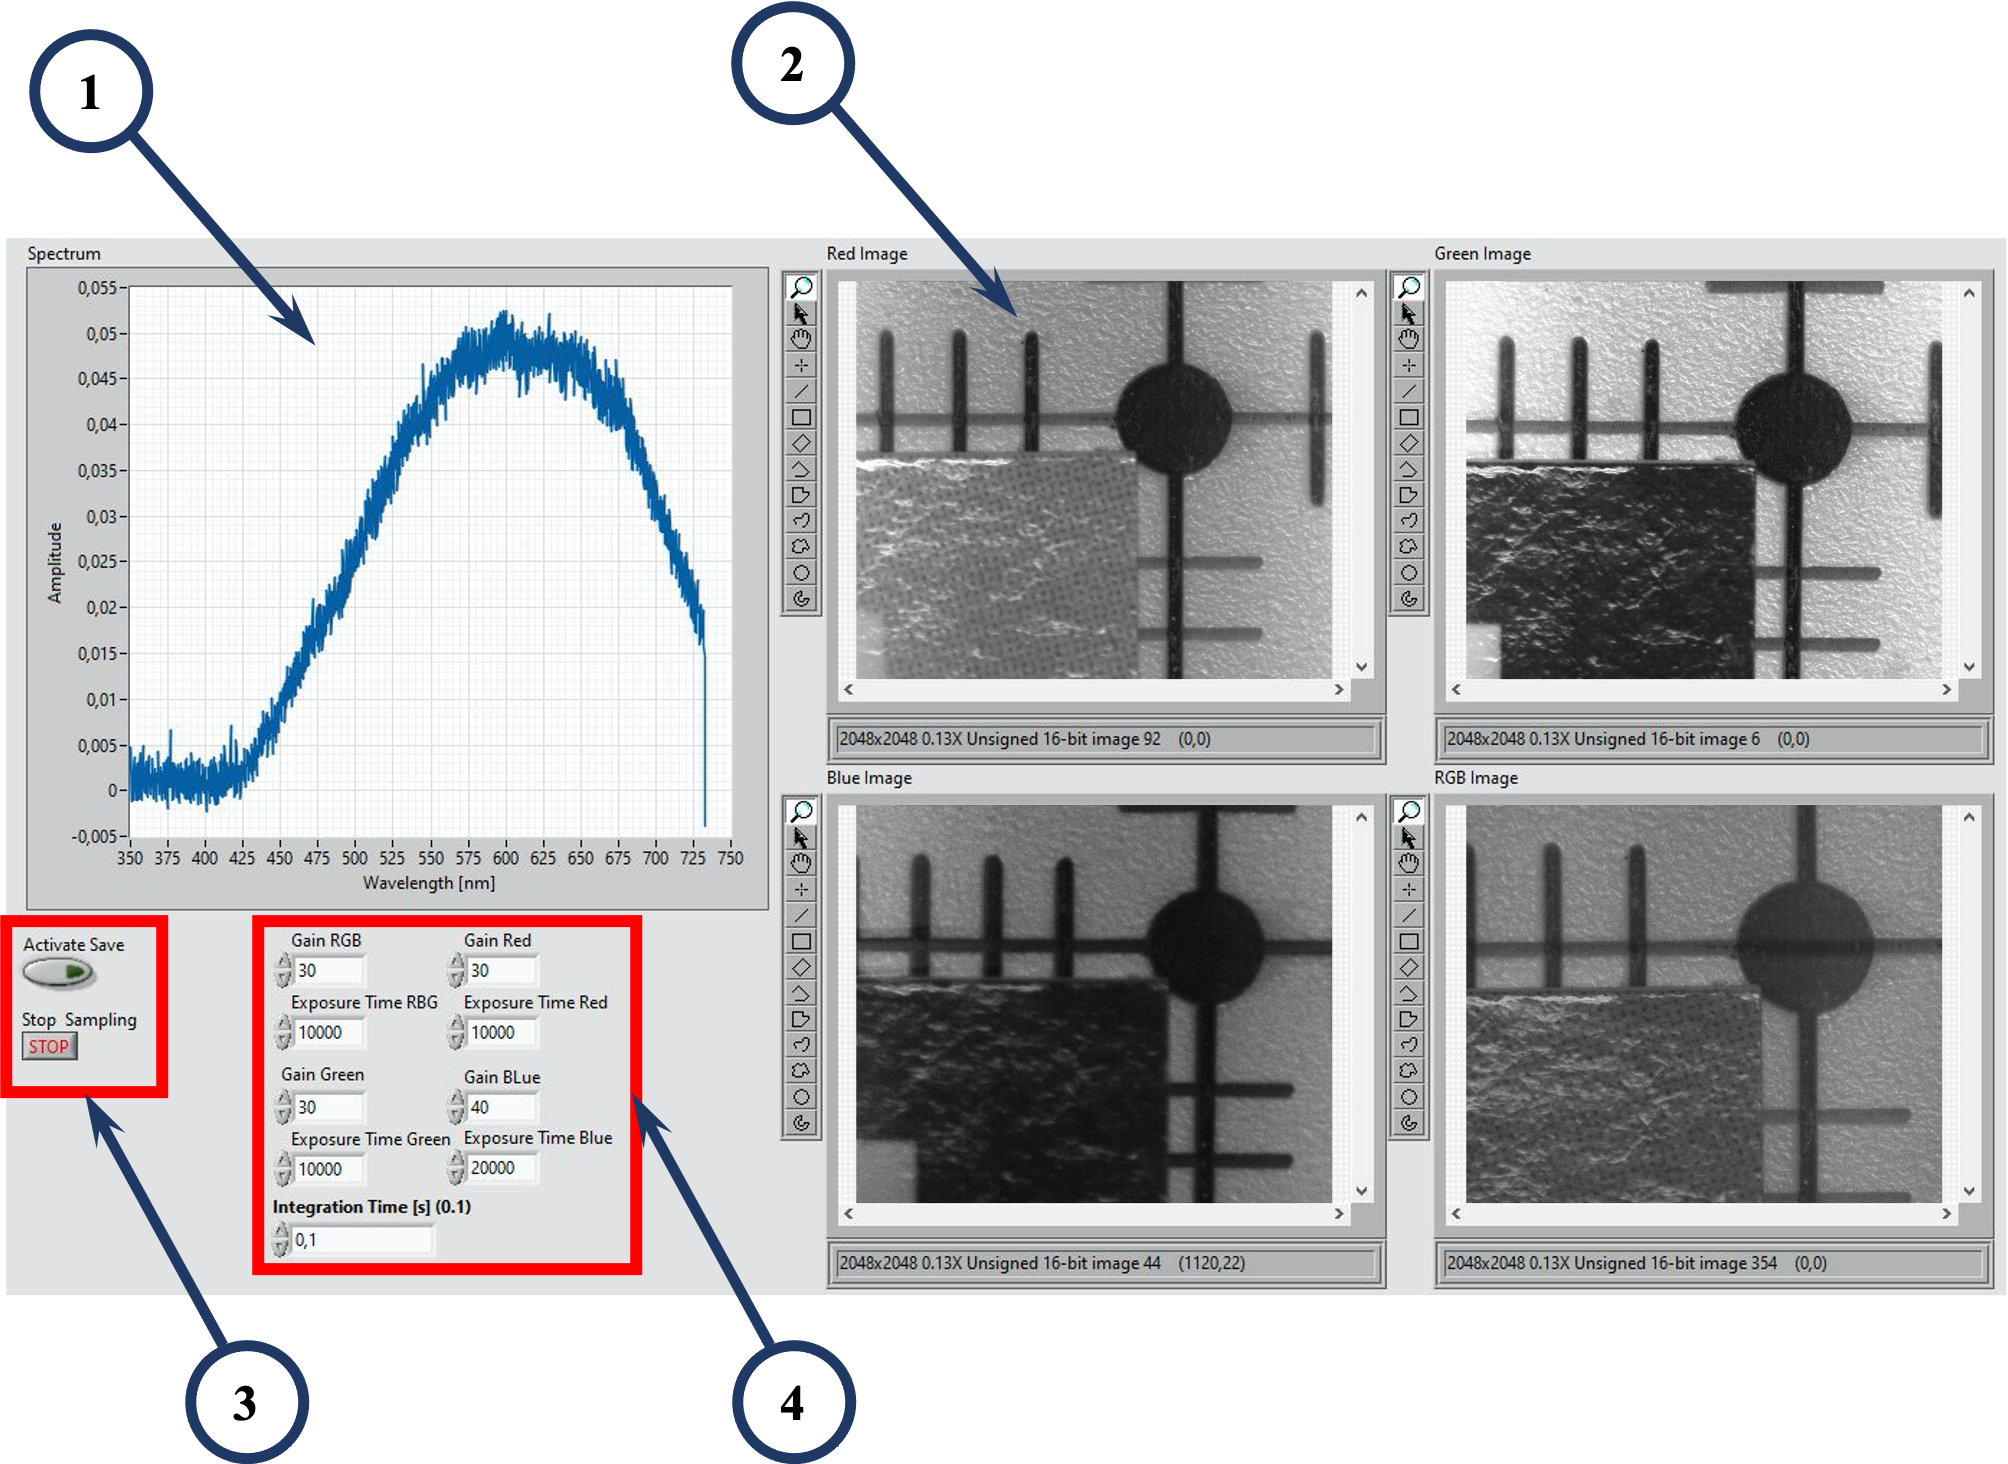
\includegraphics[width=12cm]{Pictures/Frontpanel}
\caption[Image of the LabVIEW front panel for the control of the Artificial Eye]{Image of the LabVIEW front panel for the control of the Artificial Eye: 1 - Graph with the captured spectrum, 2 - Camera images, 3 - Controls for saving and stop, 4 - Controls for device parameters}
\label{Frontpanel}
\end{center}
\end{figure}




\section{Transmission test} 
The testing of the initial setup is part of the qualification and therefore the second step in the first phase of the development of the Artificial Eye. It is shown as orange-bordered in figure \ref{ChainQuali}.

\begin{figure}[h]
\begin{center}
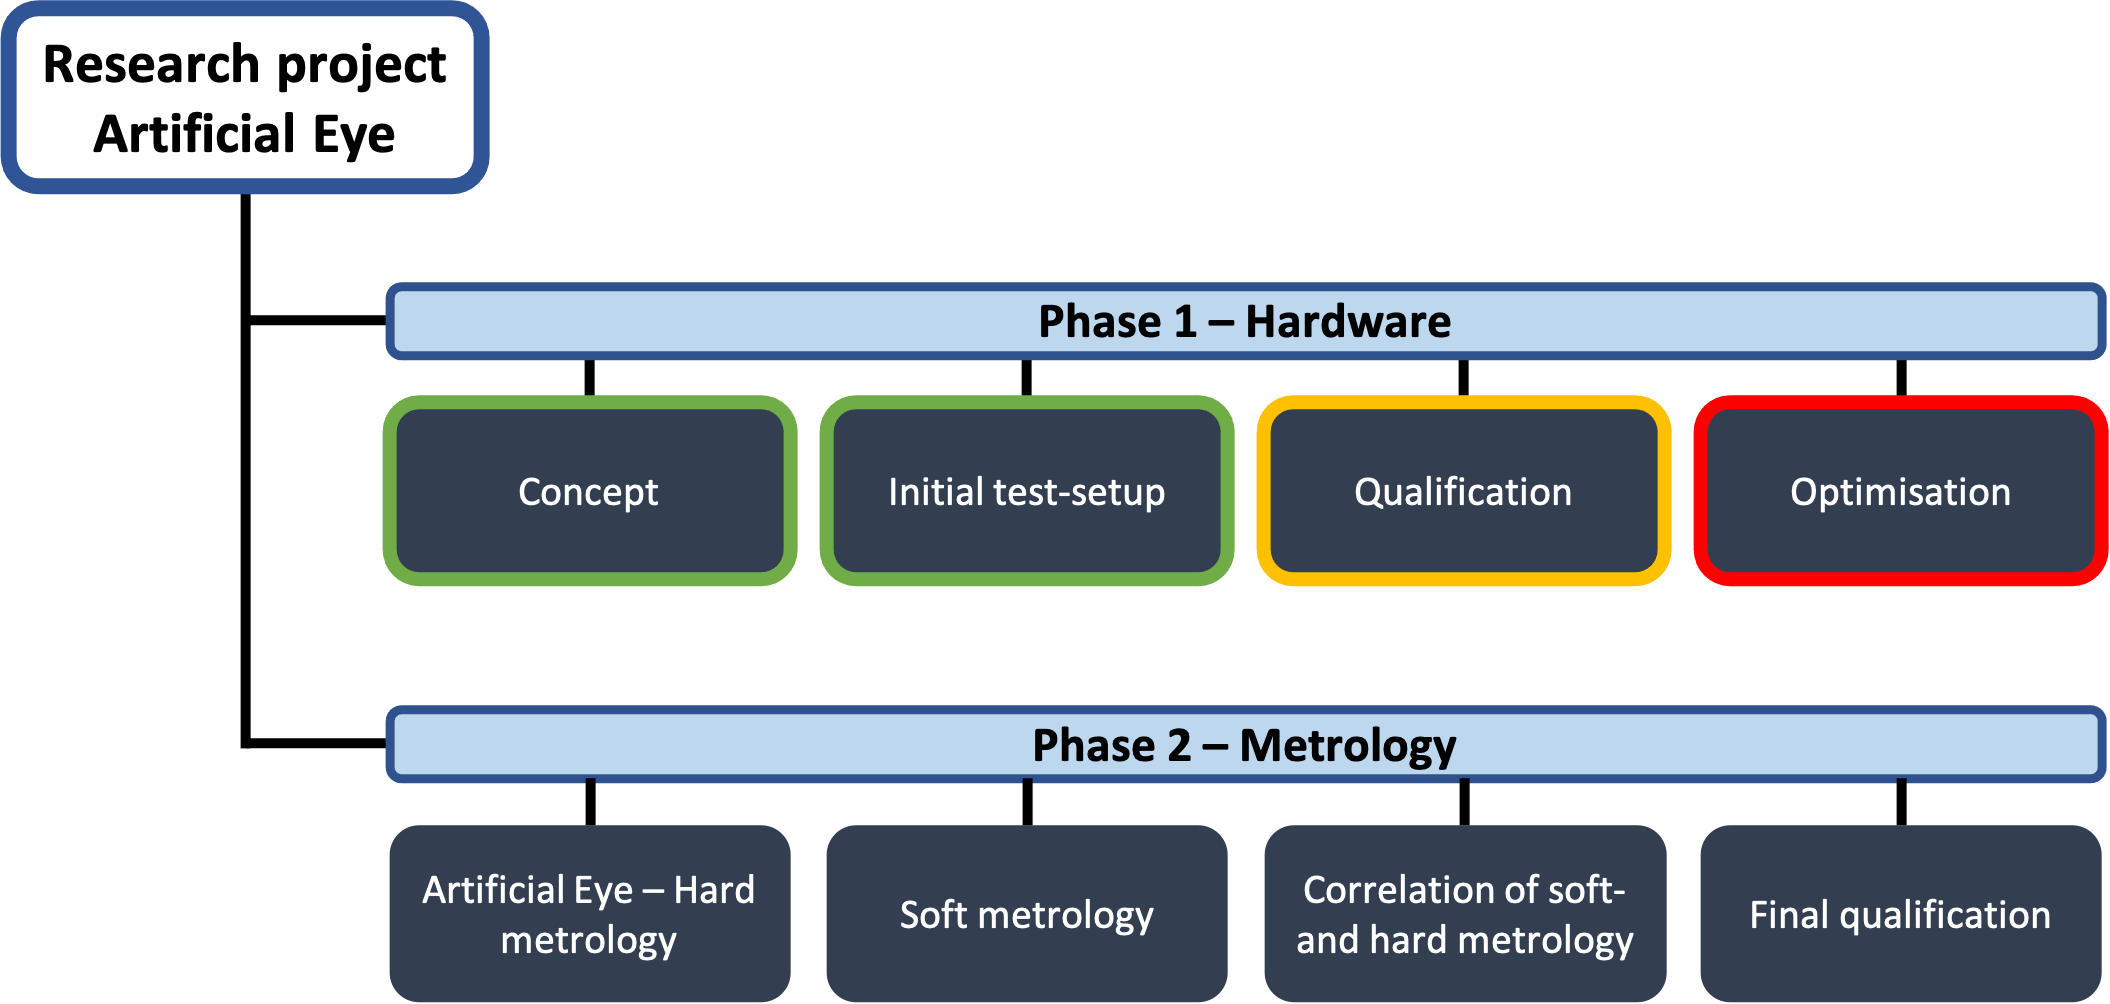
\includegraphics[width=12cm]{Pictures/ChianQuali}
\caption[Overview over the development process - Qualification]{Overview over the development process - Qualification: Green - Completed, Orange - In work, Red - Open}
\label{ChainQuali}
\end{center}
\end{figure}

This test was aimed to investigate, if the selected bandwidth of the colour filters and the transmission of the optical system is sufficient. Further the right exposure time and analog gain (amplifier) settings for the camera system need to be configured. In order to focus the camera system, a reference object was needed. During the execution of this testing series, two different types of references were used:
\subsubsection{Fine grid plate}
The reference which was used first, was a matt black rectangle made from acrylic. The acrylic was then laminated with a matt white vinyl in order to create a surface which reflects light well, but does not cause glare or direct reflections. Further, a fine grid structure was laser-etched into the white vinyl. With the acrylic as backgrounds, the grid was visible as a high contrast structure. This was used to focus the camera system and reference the position of its point of view.
\subsubsection{Illumination source}
To illuminate the reference plate, an incandescent light bulb was used. This type of light bulb provides a smooth spectrum, gradually increasing in intensity from 400 nm into the near infrared spectrum. The light intensity of the bulb was measured to be $\sim$18000 lux on the surface of the reference plate. This is roughly the intensity of daylight. The lightbulb was placed at the same hight as the optical system and the light was pointed onto the surface of the test plate at an angle of $\sim$45° in order to avoid direct reflections or glare. The spectrum of the lightbulb is shown in figure \ref{AMOLEDSpectrum}. \\

\begin{figure}
\begin{center}
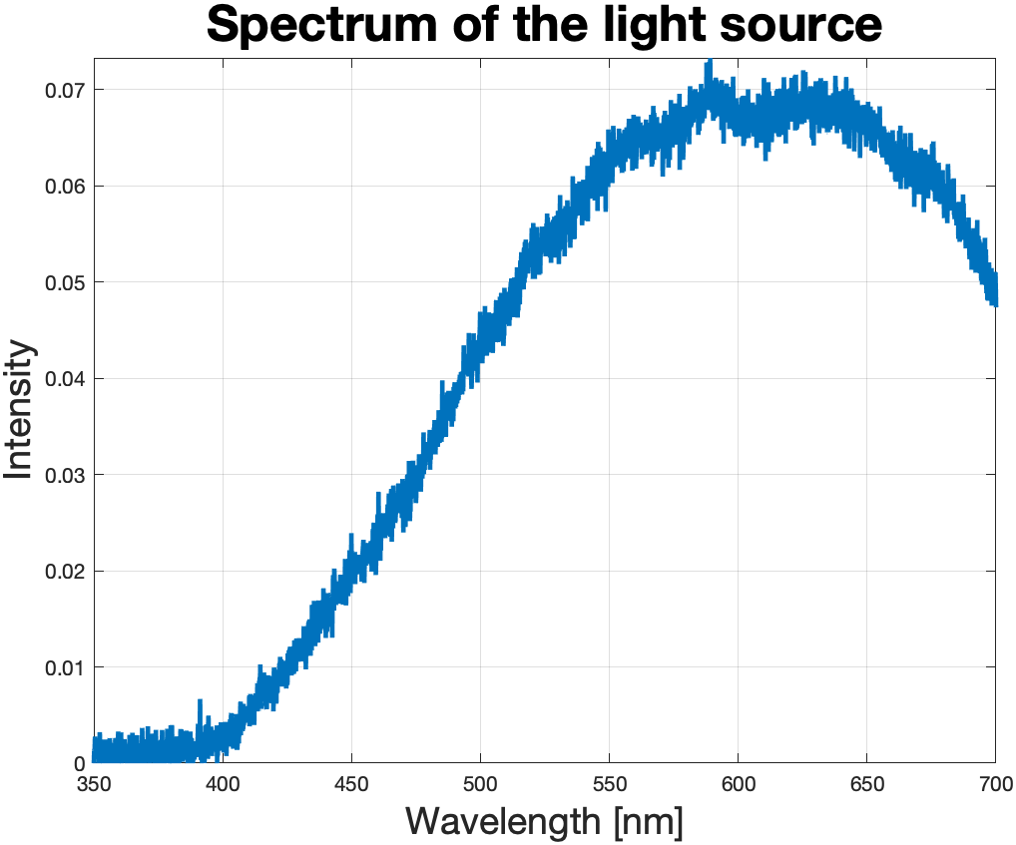
\includegraphics[width=12cm]{Pictures/AMOLEDSpectrum}
\caption[Graph showing the spectrum emitted by the incandescent light bulb]{Graph showing the spectrum emitted by the incandescent light bulb}
\label{AMOLEDSpectrum}
\end{center}
\end{figure}

In order to find a common value for the gain for all cameras in the system, the test was setup to try a variety of different values. The test was executed by setting all four cameras to the same exposure time and analog gain and saving the resulting images for evaluation. As starting values, the highest possible gain (48 dB) and an exposure time of $\frac{1}{1000}$ s was selected. The gain was then lowered in 5 dB steps. To ensure that the intensity of the illumination was consistent for all measurements, the intensity of the incoming light was measured and saved with the spectrometer. To make the data of the RGB camera comparable to the other three cameras in the setup, its was configured to output a greyscale image with a colour precision of 12 bit. This is the default output format for the three monochromatic cameras. In order to have a reference for the point where an image is too dark, a reference image was taken. This was done by adjusting the gain of the RGB camera while evaluating the brightness of the image shown in a live feed of the camera.


\section{Focus test}
The aim of this test was to ensure that all four cameras are sharing the same focal point. This is needed in order to take quick measurements without the need to readjust the focus for each of the cameras in the system. As a reference for the focus and point of view of the system, the fine grid plate was used. To measure the difference in focus and point of view between the cameras, the linear axes were used.\\
The procedure to measure the deviation between the cameras was as follows:
\begin{enumerate}
	\item The reference plate was placed in the center of the X-Y table.
	\item The connection with the camera and the Thorlabs linear axes where established. The linear axes need to be homed (referenced to the zero point of the axis)
	\item One of the cameras was selected as a reference for the remaining cameras. In this case the RGB camera was set as a reference. 
	\item The selected camera was focussed onto the reference plate.
	\item The crosshair in the center of the reference plate was moved into the FOV of the camera using the X-Y table. The inner most reference lines on the plate where aligned with the left and upper edge of the image (see figure \ref{XYZCalibSetup} right).
	\item The position of the X,Y and Z axis were noted down, as reported in the Thorlabs control software (see figure \ref{XYZCalibSetup} left). 
	\item The steps from 4. - 6. were repeated for all cameras in the system.
\end{enumerate}

\begin{figure}
\begin{center}
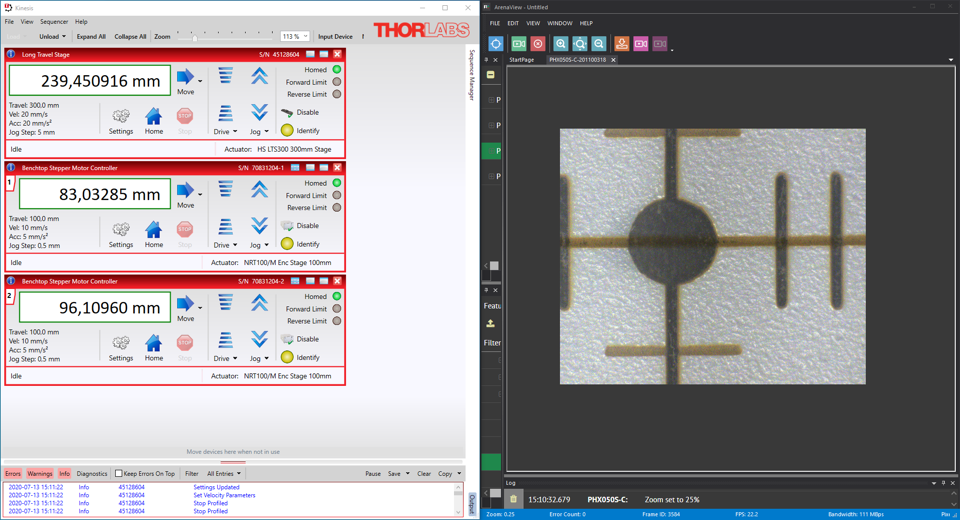
\includegraphics[width=12cm]{Pictures/XYZCalibSetup}
\caption[Picture of the process to calculate the offset of the camera system in X,Y and Z]{Picture of the process to calculate the offset of the camera system in X,Y and Z: Left - Position information of the Thorlabs linear axis system, Right - Live image of the RGB camera}
\label{XYZCalibSetup}
\end{center}
\end{figure}



\section{Resolution test}
As the human eye has a maximum resolution of 200 $\mu$m at a distance of 700 mm, it needed to be ensured, that the Artificial Eye has a similar or higher resolution. The distance of 700 mm has been chosen, because it is often used in the industry to inspect parts. One reason for that is, that 700 mm is roughly the length of an arm. Therefore it is a quick and easy solution to inspect parts at a reproducible distance in a production environment. The testing series to investigate the maximum resolution of the optical system of the Artificial Eye was conducted after the previous two tests were evaluated and therefore the initial setup of the Artificial Eye was already slightly changed. The most remarkable change to note is the different lens used in this revision of the Artificial Eye. In contrast to the old lens, the new lens features an adjustable focal length (zoom). Adjusting the focal length, widens or narrows down the FOV. At 700 mm the maximum FOV is 68x55 mm, the minimum FOV is 17x15 mm. For this reason, the resolution test has to be done for both, the maximum and minimum FOV at a viewing distance of 700mm.\\
Because there was no vertical mounting option to achieve a distance of 700 mm between the lens and the sample, the artificial eye was mounted horizontally onto the optical table. This also caused that the X-Y table could not longer be used, because it is not possible to mount it on its side. The linear axis, which was used as Z axis in the earlier setup, could still be used to adjust the focus of the system remotely.\\
To determine the maximum resolution of the optical system a calibration plate was used. This calibration plate was placed 700 mm in front of the lens of the Artificial Eye. It has a micro pattern of lines machined into its surface. The pattern consists of lines, equally spaced, with a thickness ranging 1 $\mu$m to 600 $\mu$m. Both, the complete test-setup as well as a detail of the calibration plate are shown in figure \ref{ResolutionSetup}.

\begin{figure}
\begin{center}
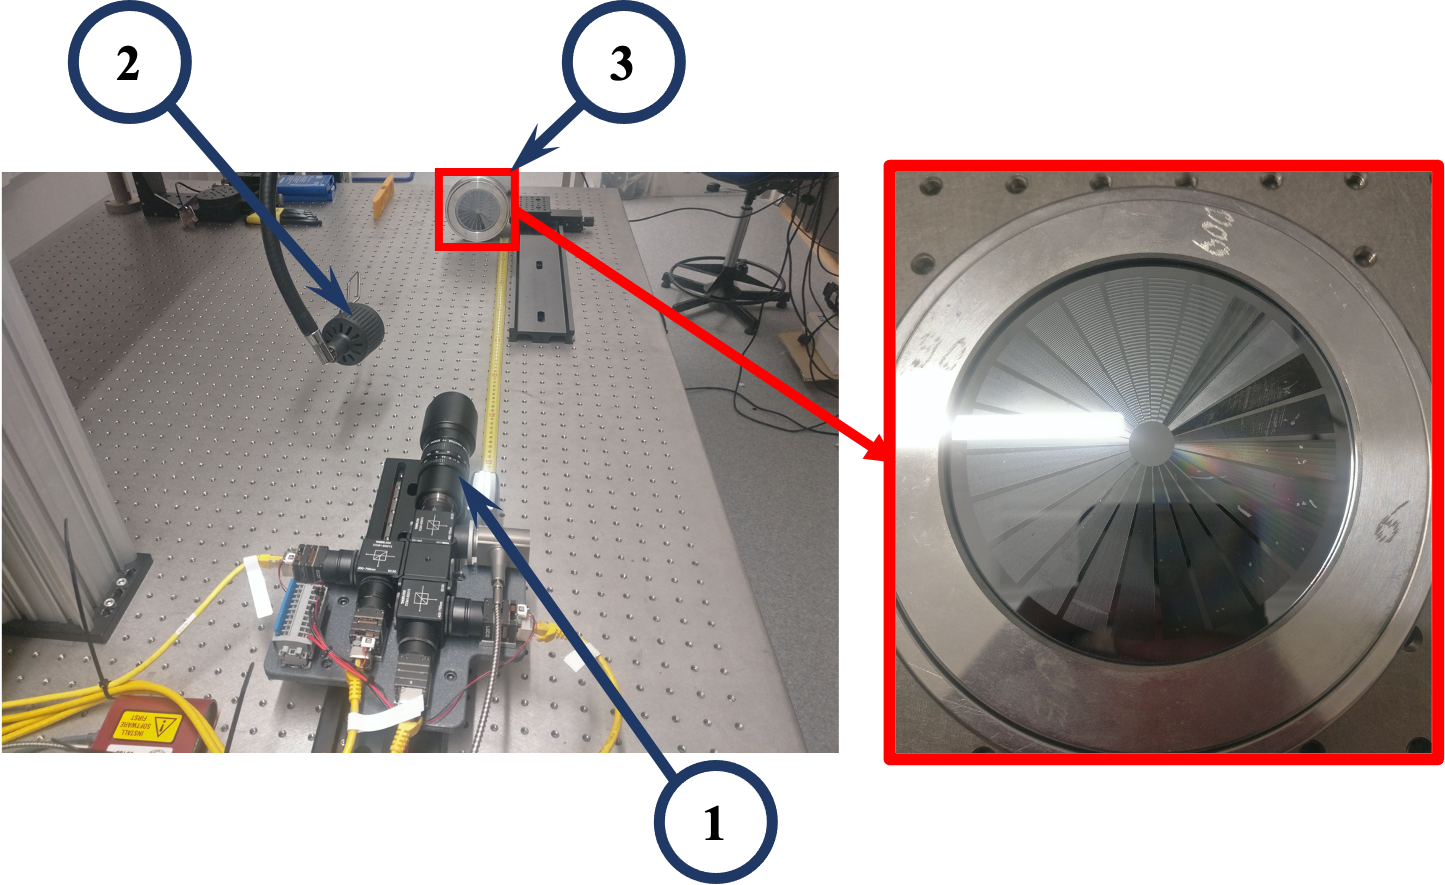
\includegraphics[width=12cm]{Pictures/ResolutionSetup}
\caption[Picture of test-setup for the minimum resolution tests]{Picture of test-setup for the minimum resolution tests}
\label{ResolutionSetup}
\end{center}
\end{figure}





